\section{Análisis del problema}
El análisis del sistema es una etapa esencial en el desarrollo de software. En esta se examinan las necesidades, requisitos y funcionalidades del sistema a implementar, ayudando a la comprensión de los usuarios finales, sus contextos de uso y los objetivos que esperan alcanzar.

\subsection{Especificación de requisitos}
Los requisitos del sistema se dividen en dos grandes categorías: funcionales y no funcionales. Estos permiten establecer de forma clara qué debe cumplir la solución propuesta para ser viable y útil. A continuación, se presenta una recopilación estructurada de los requisitos identificados.

\subsubsection{Requisitos funcionales}
Los siguientes requisitos funcionales describen las capacidades que el sistema debe implementar para cumplir con los objetivos definidos.

\begin{table}[H]
    \centering 
    \renewcommand{\arraystretch}{1.5} 
    \begin{tabular}{|l|p{12cm}|} 
        \hline 
        \rowcolor{gray!30} 
        \textbf{Código} & \textbf{RF 1.1} \\
        \hline
        \textbf{Nombre} & Generación de Imágenes Basada en Texto \\
        \hline 
        \textbf{Descripción} & Permitir la generación de imágenes a partir de descripciones textuales proporcionadas por el usuario \\
        \hline 
        \textbf{Precondición} & Acceso al sistema de generación de imágenes mediante la interfaz de usuario \\
        \hline 
        \textbf{Postcondición} & Imagen generada y visualizada en la interfaz del usuario \\
        \hline 
    \end{tabular}
    \caption{Requisito Funcional RF 1.1} 
    \label{tab:reqfun1}
\end{table}

\begin{table}[H]
    \centering 
    \renewcommand{\arraystretch}{1.5} 
    \begin{tabular}{|l|p{12cm}|} 
        \hline \rowcolor{gray!30} 
        \textbf{Código} & \textbf{RF 2.1} \\
        \hline
        \textbf{Nombre} & Compatibilidad y Escalabilidad en la JMR \\
        \hline 
        \textbf{Descripción} & Integración del sistema con la infraestructura existente en la JMR sin interrumpir otras funcionalidades \\
        \hline 
        \textbf{Precondición} & Acceso a la infraestructura actual de la JMR \\
        \hline
        \textbf{Postcondición} & El sistema de generación de imágenes opera correctamente dentro del entorno de la JMR \\ 
        \hline 
    \end{tabular} 
    \caption{Requisito Funcional RF 2.1} 
    \label{tab:reqfun2}
\end{table}

\begin{table}[H] 
    \centering 
    \renewcommand{\arraystretch}{1.5} 
    \begin{tabular}{|l|p{12cm}|} 
        \hline \rowcolor{gray!30} 
        \textbf{Código} & \textbf{RF 3.1} \\
        \hline
        \textbf{Nombre} & Gestión de Resultados de Generación de Imágenes \\
        \hline 
        \textbf{Descripción} & Permitir a los usuarios guardar y etiquetar las imágenes generadas \\
        \hline
        \textbf{Precondición} & Imagen generada y lista para almacenamiento o uso posterior \\
        \hline 
        \textbf{Postcondición} & La imagen está guardada y etiquetada correctamente \\ 
        \hline 
    \end{tabular} 
    \caption{Requisito Funcional RF 3.1} 
    \label{tab:reqfun3}
\end{table}

\begin{table}[H] 
    \centering 
    \renewcommand{\arraystretch}{1.5} 
    \begin{tabular}{|l|p{12cm}|} 
        \hline \rowcolor{gray!30}
        \textbf{Código} & \textbf{RF 4.1} \\ 
        \hline 
        \textbf{Nombre} & Interfaz de Usuario Intuitiva y Accesible \\
        \hline
        \textbf{Descripción} & Proporcionar una interfaz amigable y accesible para que los usuarios generen imágenes a partir de texto
        \\ \hline \textbf{Precondición} & Acceso al sistema de generación de imágenes a través de la interfaz \\ 
        \hline \textbf{Postcondición} & Los usuarios pueden navegar y utilizar fácilmente las funcionalidades \\
        \hline 
    \end{tabular}
    \caption{Requisito Funcional RF 4.1}
    \label{tab:reqfun4}
\end{table}


\subsubsection{Requisitos no funcionales}
Los requisitos no funcionales del sistema establecen criterios relacionados con la calidad, rendimiento, mantenimiento y accesibilidad.


\begin{table}[H] 
    \centering 
    \renewcommand{\arraystretch}{1.5} 
    \begin{tabular}{|l|p{12cm}|} 
        \hline \rowcolor{gray!30} 
        \textbf{Código} & \textbf{RNF 1} \\ 
        \hline 
        \textbf{Nombre} & Rendimiento y Eficiencia \\ 
        \hline \textbf{Descripción} & El sistema debe ser capaz de generar imágenes en un tiempo razonable, optimizando el uso de memoria y recursos de GPU \\ 
        \hline 
    \end{tabular} 
    \caption{Requisito No Funcional RNF 1: Rendimiento y Eficiencia} 
    \label{tab:reqnofun1} 
\end{table}
    
\begin{table}[H]
    \centering 
    \renewcommand{\arraystretch}{1.5} 
    \begin{tabular}{|l|p{12cm}|} 
        \hline \rowcolor{gray!30}
        \textbf{Código} & \textbf{RNF 2} \\ 
        \hline 
        \textbf{Nombre} & Mantenimiento \\ 
        \hline 
        \textbf{Descripción} & El sistema debe ser modular, permitiendo actualizaciones y mantenimiento sin afectar el funcionamiento general de la JMR \\ 
        \hline 
    \end{tabular} 
    \caption{Requisito No Funcional RNF 2: Mantenimiento} 
    \label{tab:reqnofun2}
\end{table}

\begin{table}[H] 
    \centering 
    \renewcommand{\arraystretch}{1.5} 
    \begin{tabular}{|l|p{12cm}|} 
        \hline \rowcolor{gray!30} 
        \textbf{Código} & \textbf{RNF 3} \\
        \hline 
        \textbf{Nombre} & Compatibilidad \\ 
        \hline
        \textbf{Descripción} & El sistema debe ser compatible con la infraestructura actual de la JMR. También debe permitir la integración con otros módulos o sistemas externos en el futuro. \\
        \hline 
    \end{tabular} 
    \caption{Requisito No Funcional RNF 3: Compatibilidad}
    \label{tab:reqnofun3} 
\end{table}

\begin{table}[H]
    \centering 
    \renewcommand{\arraystretch}{1.5}
    \begin{tabular}{|l|p{12cm}|} 
        \hline \rowcolor{gray!30}
        \textbf{Código} & \textbf{RNF 4} \\ 
        \hline
        \textbf{Nombre} & Experiencia de Usuario y Accesibilidad \\
        \hline \textbf{Descripción} & El sistema debe cumplir con los estándares de accesibilidad para asegurar su uso por personas con diferentes capacidades y necesidades. La interfaz debe ser responsiva y adaptarse correctamente a distintos dispositivos. \\ 
        \hline 
    \end{tabular} 
    \caption{Requisito No Funcional RNF 4: Experiencia de Usuario y Accesibilidad} 
    \label{tab:reqnofun4} 
\end{table}


\subsection{Historias de usuario}
Con el objetivo de validar y contextualizar los requisitos identificados, se han definido varias historias de usuario que ilustran cómo diferentes perfiles interactúan con el sistema. Estas historias permiten anticipar escenarios de uso realistas y orientar el diseño de funcionalidades clave.

La Tabla~\ref{tab:hu01} presenta el caso de un investigador, cuyo objetivo es experimentar con modelos de generación de imágenes y evaluar su precisión antes de integrarlos en la plataforma. Este perfil pone el foco en la calidad técnica del sistema generativo y su interoperabilidad con el entorno de recuperación visual.

\begin{table}[ht]
    \centering
    \renewcommand{\arraystretch}{1.5}
    \begin{tabular}{|>{\columncolor{gray!10}}p{4cm}|p{10cm}|}
        \hline
        \rowcolor{gray!30}
        \multicolumn{2}{|c|}{\textbf{Historia de Usuario 1}} \\
        \hline
        \textbf{Rol del Usuario} & Investigador en Inteligencia Artificial y Aprendizaje Profundo \\
        \hline
        \textbf{Necesidad} & Desarrollar y evaluar modelos de generación de imágenes a partir de texto para integrarlos en una plataforma de recuperación de información visual (JMR) \\
        \hline
        \textbf{Funcionalidades requeridas} & Implementar un modelo optimizado para generación de imágenes basada en descripciones textuales
        \\ & Evaluar la precisión y coherencia de las imágenes generadas en relación a la descripción
        \\ & Proporcionar un módulo de prueba y validación de las imágenes generadas antes de la integración en la JMR \\
        \hline
        \textbf{Beneficio} & Avanzar en las capacidades de los sistemas CBIR al permitir búsquedas más naturales y accesibles basadas en texto, mejorando la precisión en la recuperación de imágenes \\
        \hline
    \end{tabular}
    \caption{Historia de Usuario 1}
    \label{tab:hu01}
\end{table}

La Tabla~\ref{tab:hu02} aborda el punto de vista del administrador de la JMR, responsable de integrar y mantener el sistema dentro de una infraestructura ya existente. Aquí, los aspectos de compatibilidad, usabilidad y estabilidad del sistema cobran especial relevancia.

\begin{table}[ht]
    \centering
    \renewcommand{\arraystretch}{1.5}
    \begin{tabular}{|>{\columncolor{gray!10}}p{4cm}|p{10cm}|}
        \hline
        \rowcolor{gray!30}
        \multicolumn{2}{|c|}{\textbf{Historia de Usuario 2}} \\
        \hline
        \textbf{Rol del Usuario} & Administrador de la JMR \\
        \hline
        \textbf{Necesidad} & Integrar un sistema de generación de imágenes a partir de texto que sea compatible con la infraestructura actual de la JMR \\
        \hline
        \textbf{Funcionalidades requeridas} & Implementar una interfaz de usuario intuitiva que permita a los usuarios ingresar descripciones textuales para la generación de imágenes
        \\ & Asegurar la compatibilidad y escalabilidad del módulo de generación de imágenes dentro de la infraestructura existente de la JMR
        \\ & Supervisar el rendimiento y la estabilidad del sistema para garantizar una experiencia fluida al usuario \\
        \hline
        \textbf{Beneficio} & Ofrecer un sistema CBIR basado en texto que potencie las funcionalidades de la JMR, proporcionando una experiencia avanzada y personalizada de búsqueda visual para los usuarios \\
        \hline
    \end{tabular}
    \caption{Historia de Usuario 2}
    \label{tab:hu02}
\end{table}

Por último, en la Tabla~\ref{tab:hu03} se presenta al usuario final, quien se beneficia directamente de la generación de imágenes como forma de consulta. Este perfil prioriza la facilidad de uso, la calidad de los resultados generados y la capacidad de aplicar el sistema en contextos reales.

\begin{table}[ht]
    \centering
    \renewcommand{\arraystretch}{1.5}
    \begin{tabular}{|>{\columncolor{gray!10}}p{4cm}|p{10cm}|}
        \hline
        \rowcolor{gray!30}
        \multicolumn{2}{|c|}{\textbf{Historia de Usuario 3}} \\
        \hline
        \textbf{Rol del Usuario} & Usuario Final del Sistema de Recuperación de Imágenes \\
        \hline
        \textbf{Necesidad} & Utilizar un sistema que permita recuperar imágenes relevantes basadas en descripciones textuales para apoyar investigaciones o proyectos específicos \\
        \hline
        \textbf{Funcionalidades requeridas} & Generar imágenes basadas en consultas textuales específicas que describan escenarios, objetos o características
        \\ & Acceder a una interfaz intuitiva que permita introducir consultas de texto y visualizar resultados de forma rápida y precisa
        \\ & Poder almacenar o compartir las imágenes generadas para análisis posterior o trabajo colaborativo \\
        \hline
        \textbf{Beneficio} & Facilitar el acceso a imágenes específicas mediante descripciones, eliminando la necesidad de búsquedas visuales tradicionales y agilizando los procesos de investigación y aprendizaje \\
        \hline
    \end{tabular}
    \caption{Historia de Usuario 3}
    \label{tab:hu03}
\end{table}

El conjunto de estas historias permite cubrir una perspectiva holística del sistema: desde el desarrollo técnico hasta el uso práctico. A continuación, se presenta una tabla que muestra la correspondencia entre los requisitos definidos y las historias de usuario que los motivan. Esta relación asegura que cada funcionalidad o característica del sistema responde directamente a una necesidad concreta, lo que refuerza la coherencia y la orientación al usuario del diseño.


\begin{table}[H]
    \centering
    \renewcommand{\arraystretch}{1.4}
    \begin{tabular}{|c|p{6cm}|c|}
        \hline
        \rowcolor{gray!30}
        \textbf{Código del Requisito} & \textbf{Descripción resumida} & \textbf{Historia de Usuario} \\
        \hline
        RF 1.1 & Generación de imágenes a partir de texto & HU1, HU3 \\
        \hline
        RF 2.1 & Integración con la plataforma JMR & HU2 \\
        \hline
        RF 3.1 & Almacenamiento y etiquetado de imágenes & HU3 \\
        \hline
        RF 4.1 & Interfaz de usuario intuitiva y accesible & HU2, HU3 \\
        \hline
        RNF 1 & Eficiencia y rendimiento en la generación & HU1, HU2 \\
        \hline
        RNF 2 & Mantenimiento modular del sistema & HU2 \\
        \hline
        RNF 3 & Compatibilidad con la infraestructura JMR & HU2 \\
        \hline
        RNF 4 & Accesibilidad y experiencia de usuario & HU3 \\
        \hline
    \end{tabular}
    \caption{Relación entre requisitos y sus historias de usuario}
    \label{tab:req-hu}
\end{table}


\subsection{Modelo de caso de uso}
El modelo de caso de uso presentado en la Figura~\ref{fig:caso-uso} muestra las interacciones principales entre los actores y las funcionalidades del sistema de generación de imágenes a partir de texto integrado en la plataforma JMR. Este diagrama incluye la generación de imágenes desde una descripción textual, la visualización y personalización de resultados, el uso opcional de descriptores avanzados ofrecidos por la JMR, y la posibilidad de guardar o reutilizar las imágenes generadas.

Los actores principales identificados en el sistema son:
\begin{itemize}
    \item \textbf{Usuario final:} persona que introduce una descripción textual y visualiza o descarga las imágenes generadas.
    \item \textbf{Administrador:} encargado de configurar parámetros del sistema, gestionar el uso del generador y mantener la integración con la plataforma JMR.
\end{itemize}

Este modelo permite delimitar con claridad las funcionalidades accesibles para cada tipo de usuario y ha servido como base para la extracción de requisitos funcionales. Además, constituye un punto de partida para el desarrollo de los diagramas de secuencia y de actividad, que detallan la lógica interna del sistema y el flujo de datos entre sus componentes.

\begin{figure}[H]
    \centering
    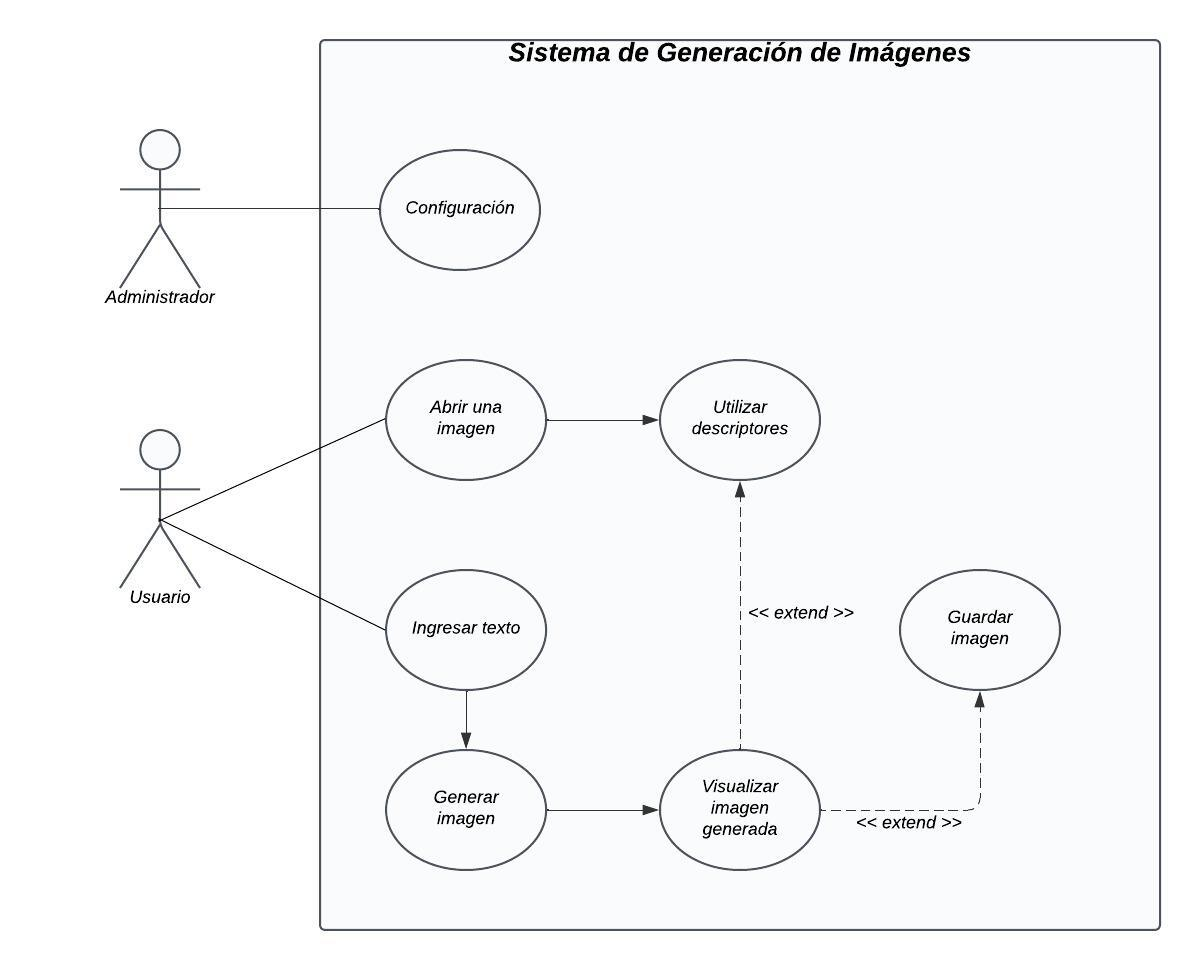
\includegraphics[width=1.0\textwidth]{diagramas/caso_uso}
    \caption{Diagrama de caso de uso}
    \label{fig:caso-uso}
\end{figure}


\subsection{Modelos de comportamiento}
Los modelos de comportamiento permiten representar la lógica dinámica del sistema, mostrando cómo interactúan sus componentes y usuarios en tiempo real. A través de diagramas de secuencia y un diagrama de actividad, se describen distintos flujos clave: desde la generación de imágenes a partir de texto, hasta la gestión de resultados y el entrenamiento del modelo.

Estos diagramas permiten visualizar cómo se comunican los distintos módulos (como la API de generación, el módulo de entrenamiento o los sistemas de almacenamiento), y ayudan a validar que las funcionalidades implementadas siguen una lógica coherente con los requisitos definidos.

\subsubsection{Diagramas de secuencia}

Los diagramas de secuencia representan interacciones temporales entre los actores y los componentes internos del sistema, reflejando cómo se produce la comunicación entre ellos en distintos escenarios clave. A continuación, se presentan los diagramas más relevantes que ilustran la lógica de funcionamiento de cada flujo:

\begin{itemize}
    \item La Figura~\ref{fig:diagrama-descriptores} muestra el proceso mediante el cual un usuario selecciona un descriptor visual desde la interfaz del sistema. El flujo se inicia con la acción del actor, quien elige el descriptor deseado; esta solicitud se transmite al controlador de descriptores, que se encarga de procesarla y consultar al módulo correspondiente. El módulo aplica el descriptor y devuelve el resultado, que finalmente se muestra al usuario.
    
    \item La Figura~\ref{fig:diagrama-generar} detalla la generación de una imagen a partir de una descripción textual. El actor introduce un prompt desde la interfaz, que es enviado al controlador de generación. Este comunica la petición a la API de generación, la cual procesa el texto y genera la imagen correspondiente. El resultado es devuelto y mostrado al usuario.

    \item La Figura~\ref{fig:diagrama-guardar} representa el proceso de almacenamiento de una imagen generada. El usuario elige la opción de guardar y proporciona una ruta de destino. La solicitud es gestionada por el controlador de imágenes, que delega en el sistema de archivos local la escritura del fichero. Una vez finalizado el proceso, se notifica al usuario.

    \item La Figura~\ref{fig:diagrama-coco} ilustra el procedimiento para la obtención y preparación de datos desde el conjunto COCO. El sistema de gestión de datos solicita al servidor las imágenes y descripciones, las cuales se obtienen desde la base de datos. Una vez recuperados, los datos son preprocesados y enviados de vuelta listos para ser utilizados en el entrenamiento.

    \item La Figura~\ref{fig:diagrama-secuencia-entrenamiento} muestra el flujo correspondiente al entrenamiento de un modelo generativo. El sistema de procesamiento de datos envía los datos al servidor de entrenamiento, donde se realiza el preprocesamiento. Posteriormente, el servidor entrena el modelo y almacena los resultados en la base de datos de modelos. Al finalizar, se notifica el éxito del entrenamiento.

    \item Finalmente, la Figura~\ref{fig:diagrama-secuencia-perdidas} detalla el cálculo y monitorización de pérdidas durante el proceso de entrenamiento. A partir de la solicitud del usuario, se inicia el entrenamiento y se registran las pérdidas del generador y el discriminador. Estos valores se visualizan gráficamente y se devuelven al sistema como salida.
\end{itemize}

\begin{figure}[H]
    \centering
    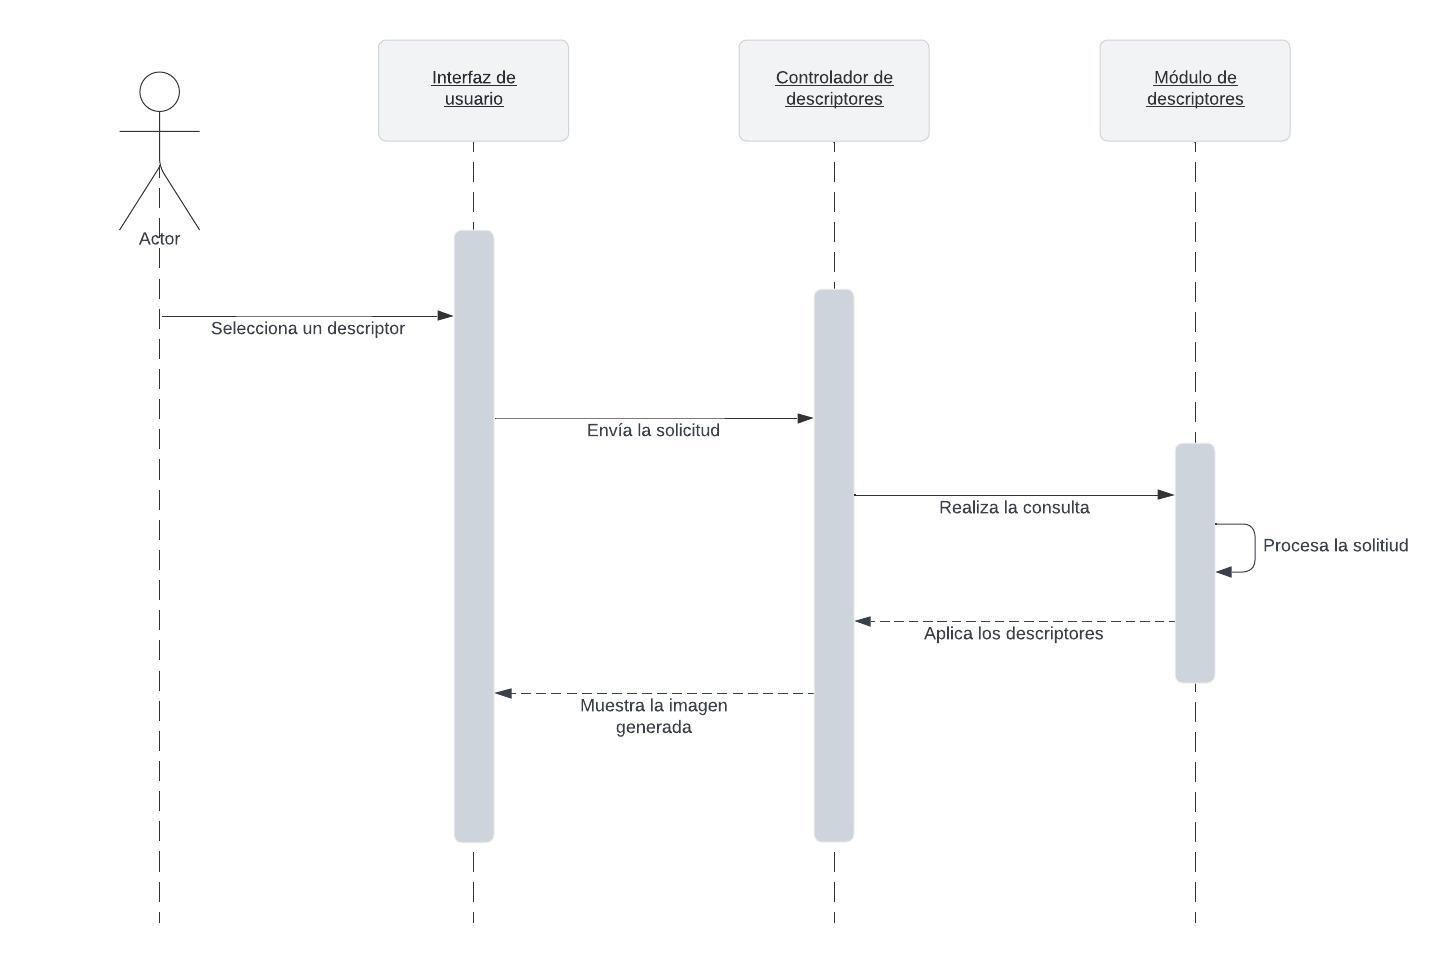
\includegraphics[width=0.8\textwidth]{diagramas/secuencia/diagrama_descriptores}
    \caption{Diagrama de secuencia del uso de descriptores}
    \label{fig:diagrama-descriptores}
\end{figure}

\begin{figure}[H]
    \centering
    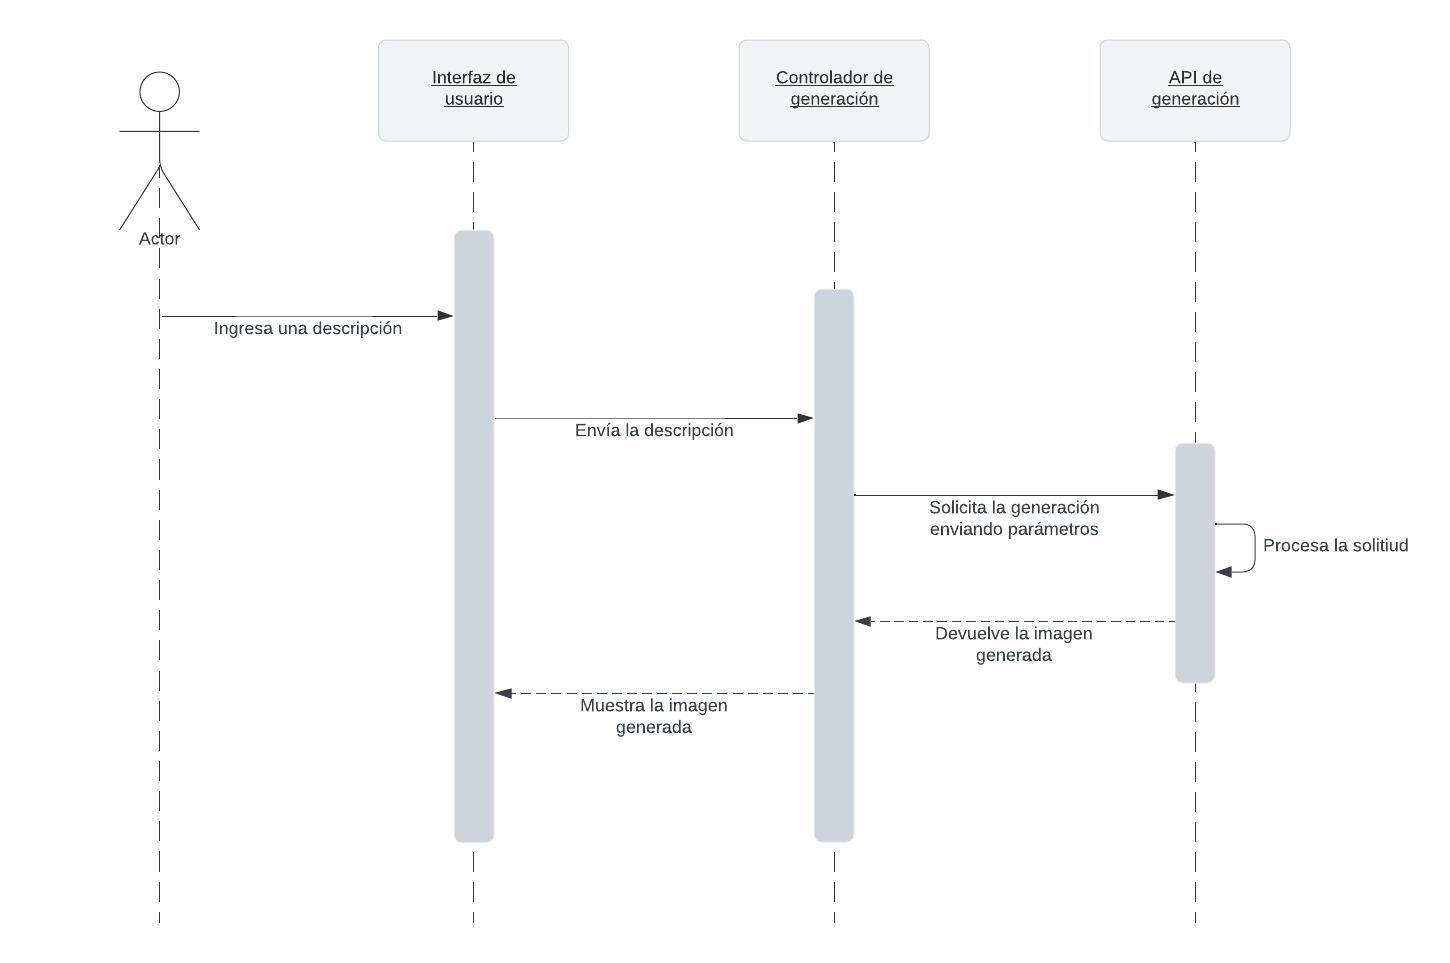
\includegraphics[width=0.8\textwidth]{diagramas/secuencia/diagrama_generar}
    \caption{Diagrama de secuencia de la generación de una imagen}
    \label{fig:diagrama-generar}
\end{figure}

\begin{figure}[H]
    \centering
    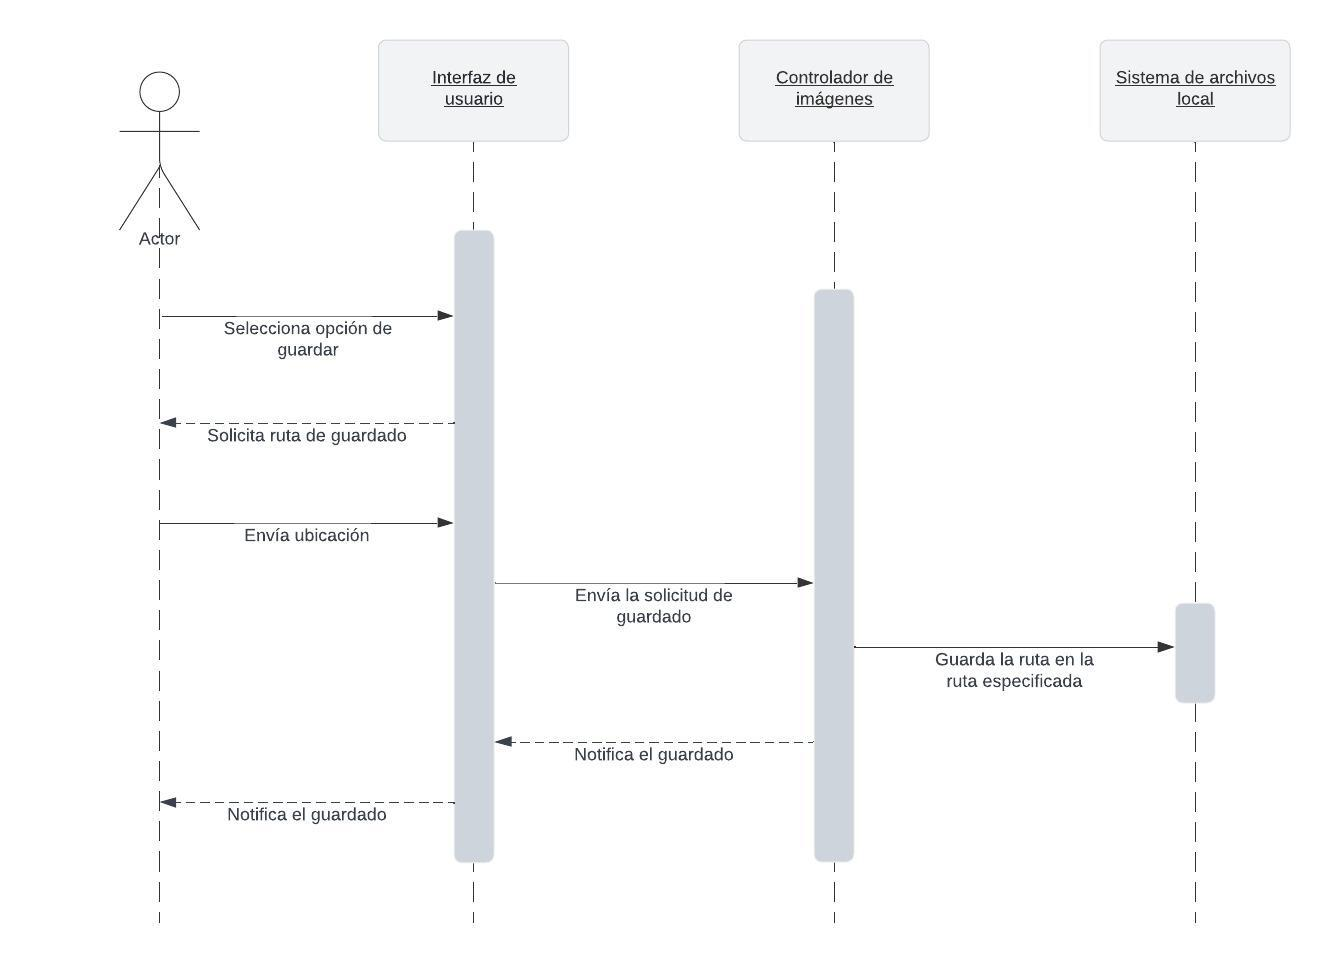
\includegraphics[width=0.8\textwidth]{diagramas/secuencia/diagrama_guardar}
    \caption{Diagrama de secuencia del guardado de una imagen}
    \label{fig:diagrama-guardar}
\end{figure}

\begin{figure}[H]
    \centering
    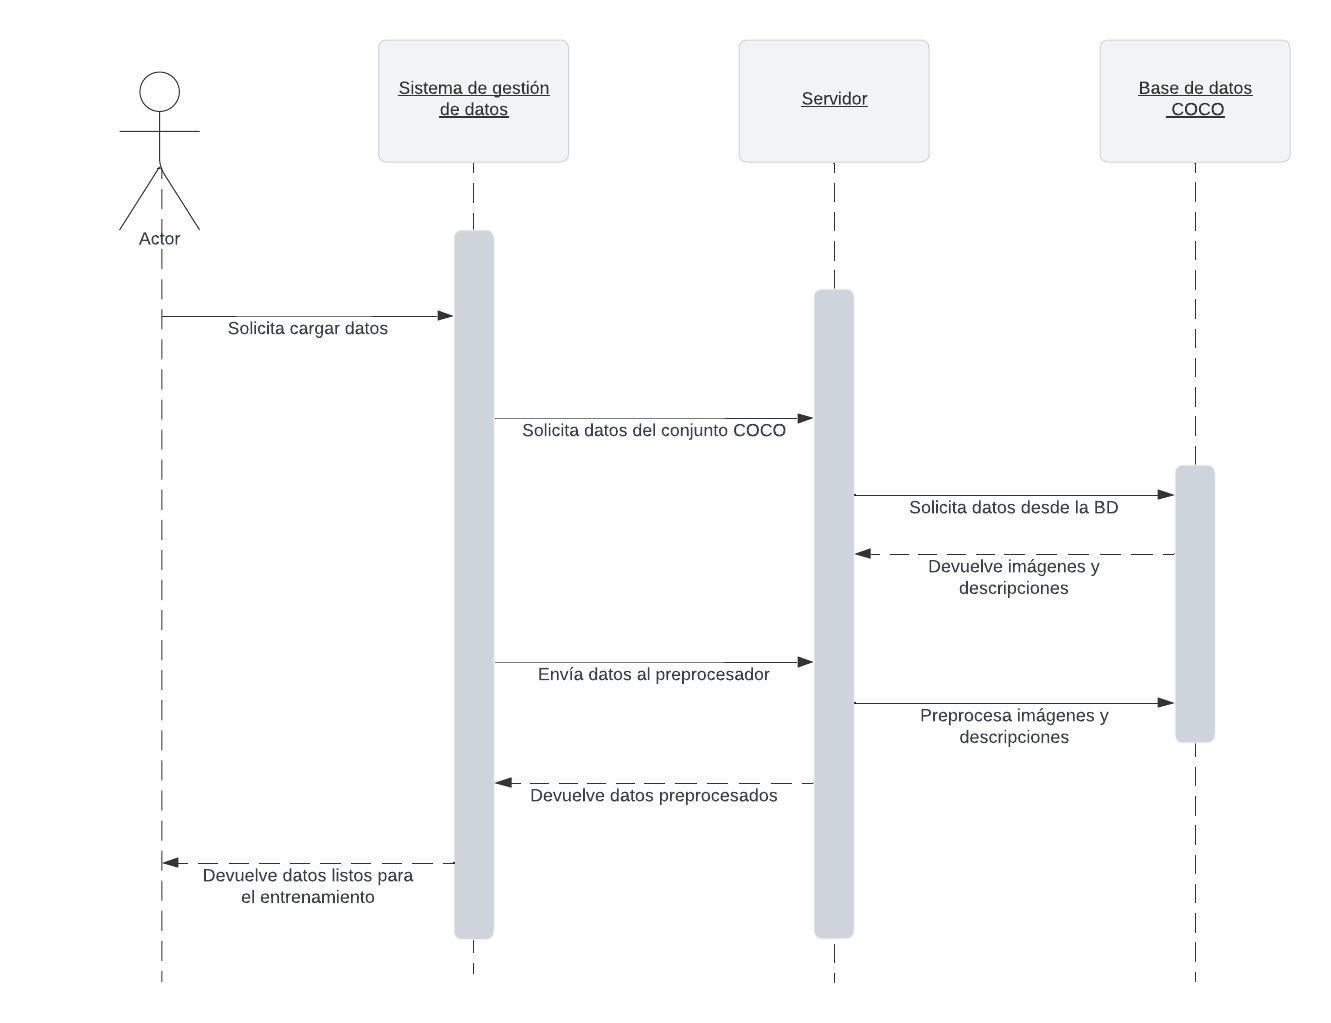
\includegraphics[width=0.8\textwidth]{diagramas/secuencia/diagrama_coco}
    \caption{Diagrama de secuencia del conjunto de datos COCO}
    \label{fig:diagrama-coco}
\end{figure}

\begin{figure}[H]
    \centering
    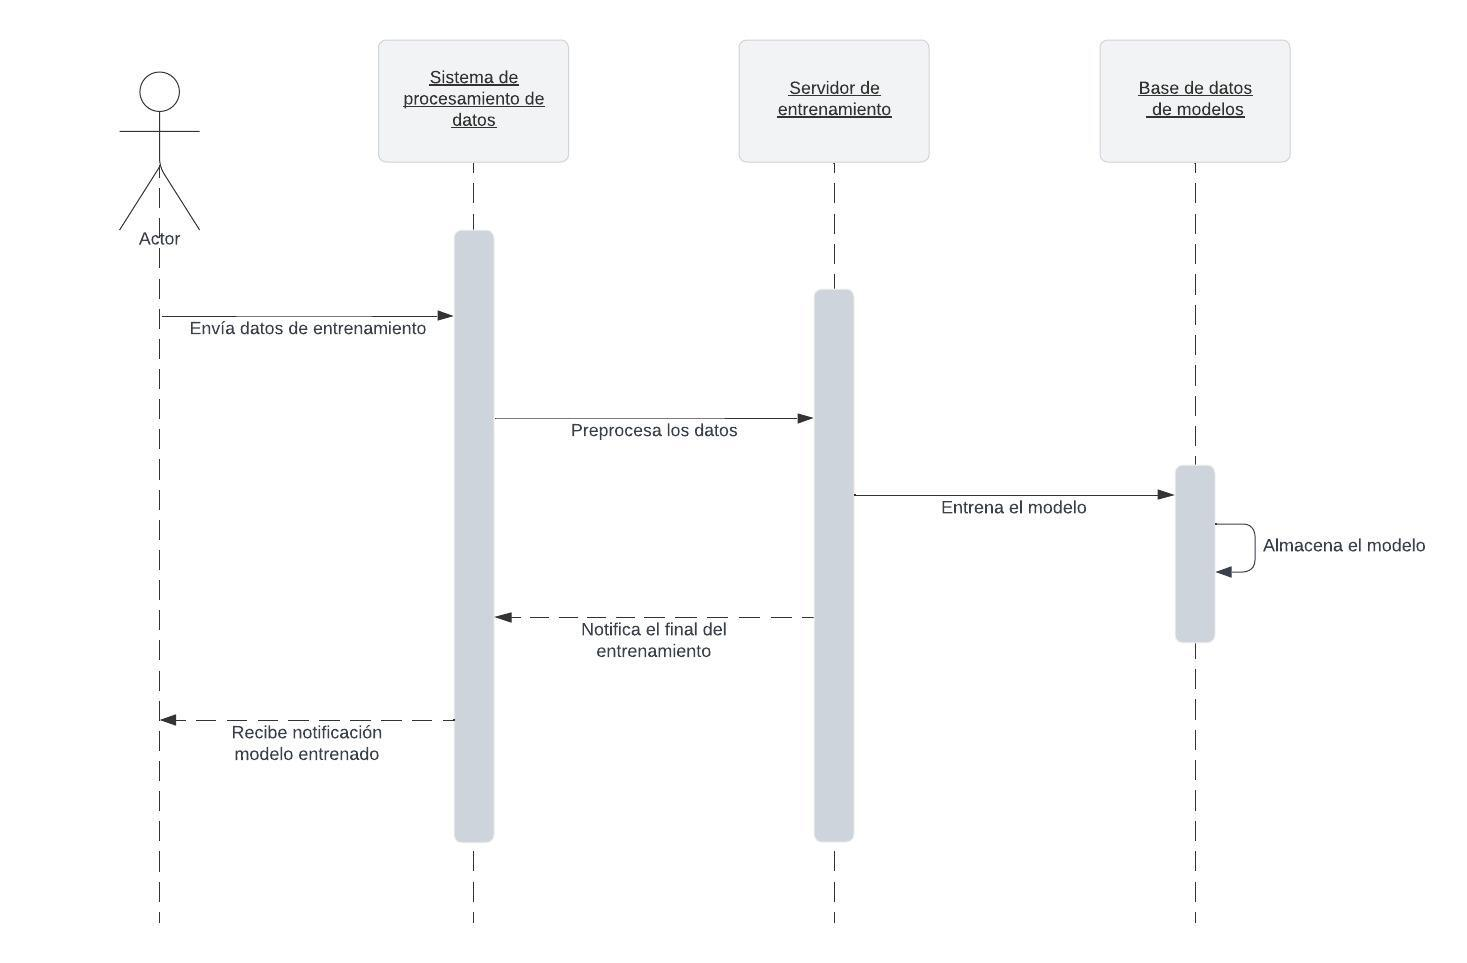
\includegraphics[width=0.8\textwidth]{diagramas/secuencia/diagrama_entrenamiento}
    \caption{Diagrama de secuencia del entrenamiento}
    \label{fig:diagrama-secuencia-entrenamiento}
\end{figure}

\begin{figure}[H]
    \centering
    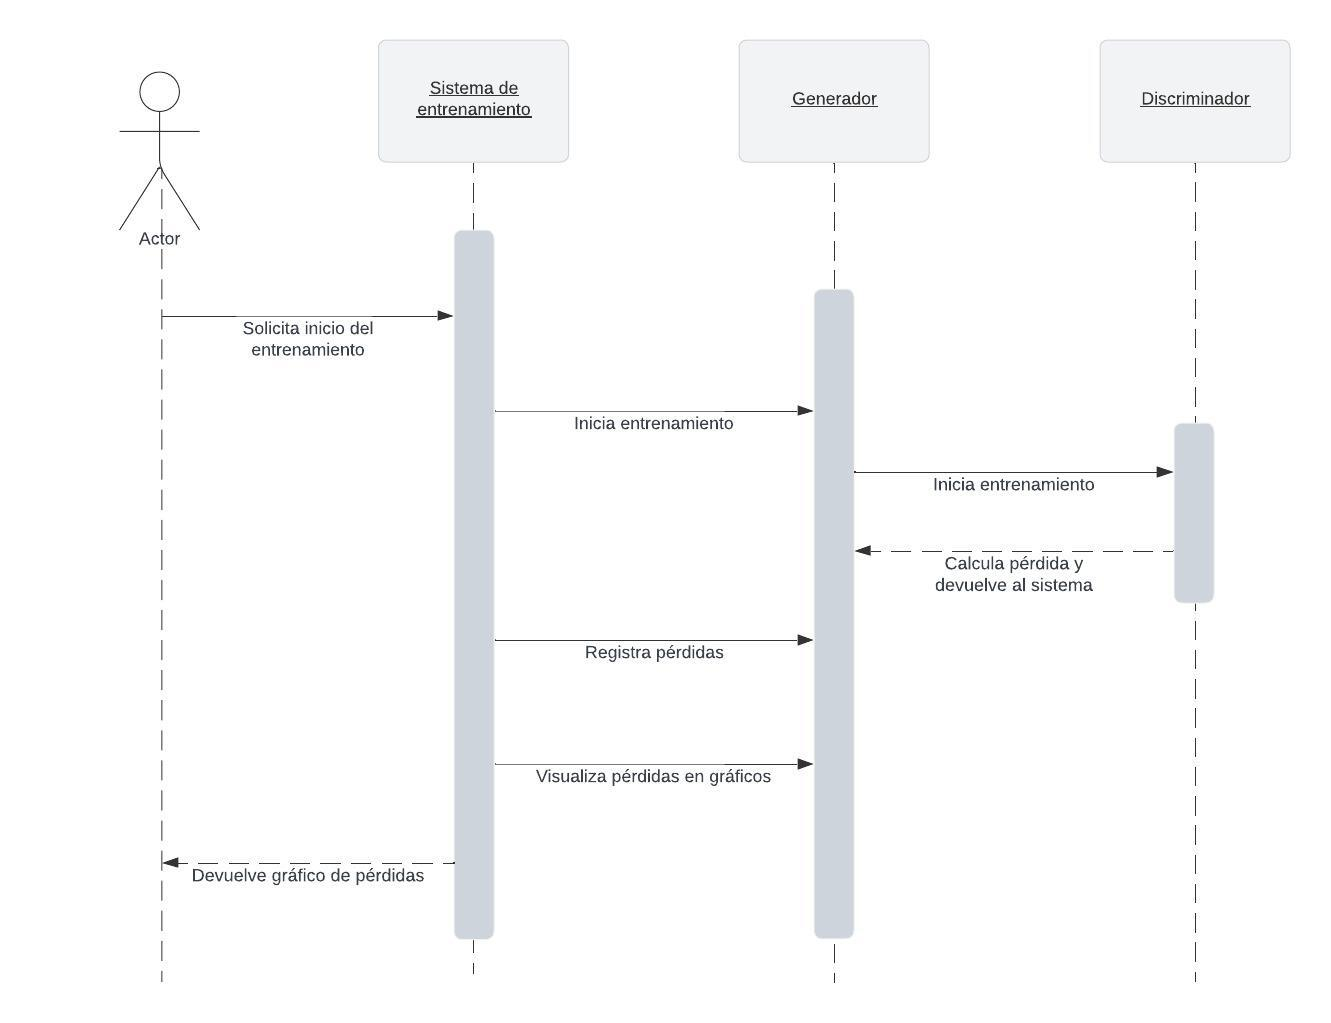
\includegraphics[width=0.8\textwidth]{diagramas/secuencia/diagrama_perdidas}
    \caption{Diagrama de secuencia de pérdidas}
    \label{fig:diagrama-secuencia-perdidas}
\end{figure}

\subsubsection{Trazabilidad entre casos de uso, historias de usuario y requisitos}
Para asegurar la coherencia entre el análisis de requisitos, las historias de usuario y los casos de uso definidos, se ha elaborado una matriz de trazabilidad. Esta permite verificar que cada funcionalidad descrita en los casos de uso responde a una necesidad real expresada por los usuarios, y que cuenta con respaldo técnico mediante los requisitos previamente establecidos. De este modo, se garantiza una cobertura completa de los objetivos del sistema y se facilita su validación durante las fases de diseño e implementación.


\begin{table}[H]
    \centering
    \renewcommand{\arraystretch}{1.4}
    \begin{tabular}{|c|p{4.5cm}|p{2.5cm}|p{4cm}|}
        \hline
        \rowcolor{gray!30}
        \textbf{Caso de Uso} & \textbf{Descripción} & \textbf{Historias de Usuario} & \textbf{Requisitos} \\
        \hline
        CU1 & Generar imagen desde texto & HU1, HU3 & RF 1.1, RF 4.1, RNF 1, RNF 4 \\
        \hline
        CU2 & Visualizar y guardar resultados & HU3 & RF 3.1, RF 4.1, RNF 4 \\
        \hline
        CU3 & Configurar y mantener el sistema & HU2 & RF 2.1, RNF 2, RNF 3 \\
        \hline
        CU4 & Entrenamiento y evaluación de modelo & HU1 & RNF 1, RNF 2 \\
        \hline
        CU5 & Selección y aplicación de descriptores & HU2 & RF 2.1, RNF 3 \\
        \hline
    \end{tabular}
    \caption{Relación entre casos de uso, historias de usuario y requisitos}
    \label{tab:trazabilidad-casos-hu-req}
\end{table}

\subsubsection{Diagrama de actividad}
La Figura~\ref{fig:diagrama-actividad} representa el flujo general de uso del sistema desde la perspectiva del usuario final. Este diagrama describe el camino típico que sigue un usuario: desde introducir una descripción, visualizar los resultados generados, hasta decidir si desea guardar o personalizar la imagen. También permite identificar puntos de decisión y posibles bifurcaciones en el flujo de interacción.

El diagrama está dividido en tres columnas que representan los principales participantes del flujo: el Usuario, la Aplicación local y la API de generación. El proceso comienza con la ejecución de la aplicación, seguida de la carga de los datos necesarios. En caso de error durante esta etapa, el sistema informa al usuario y finaliza el flujo.

Si la carga es exitosa, el usuario introduce una descripción textual que es recogida por la aplicación y enviada a la API. Esta procesa la información y genera una imagen, la cual es enviada codificada de vuelta a la aplicación local. Si hay un error en la generación, el sistema puede manejarlo y reportarlo.

La aplicación decodifica la información recibida, muestra la imagen generada y permite al usuario visualizarla. Finalmente, el usuario puede aplicar descriptores adicionales sobre la imagen, completando así el ciclo de interacción. Este flujo refleja de manera clara y estructurada la experiencia de uso prevista para la funcionalidad principal del sistema.


\begin{figure}[H]
    \centering
    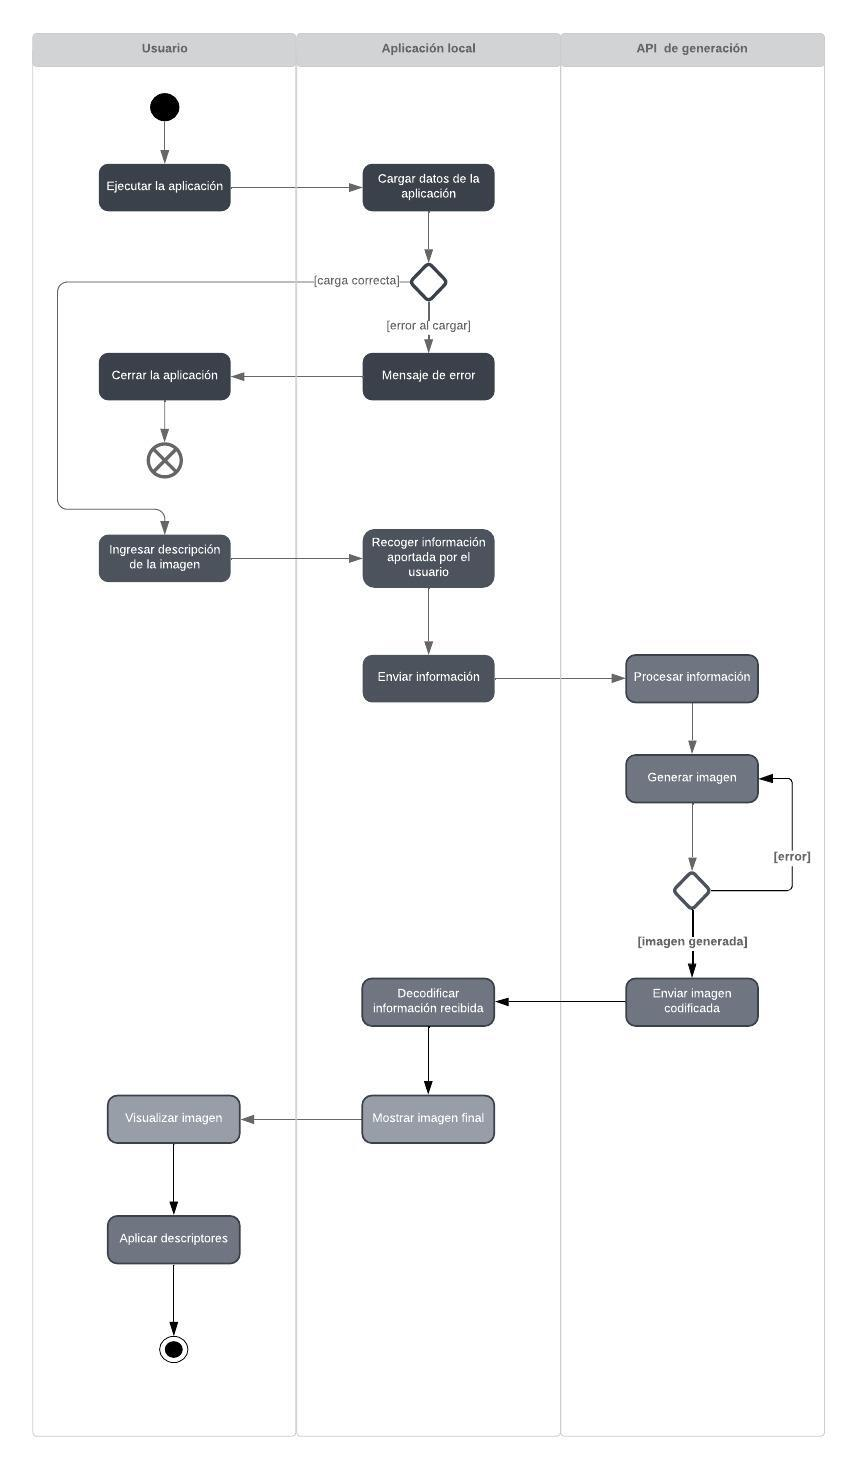
\includegraphics[width=0.8\textwidth]{diagramas/diagrama_actividad}
    \caption{Diagrama de actividad general del sistema}
    \label{fig:diagrama-actividad}
\end{figure}


